\chapter{Methodology}
\label{chap:methodology}
This chapter presents a general framework for upholding Service Level Objectives (SLOs) in distributed stream processing pipelines deployed in edge computing environments. The methodology addresses the central research question \ref{sec:research-question} of this thesis. To provide an answer, this thesis proposes a unified architecture that combines parallel stream processing with Active Inference (AIF)–based adaptive control. This architecture is designed to elastically adjust system behavior to uphold SLOs in the face of limited computational resources and dynamic workloads. It is designed to be generic, extensible, and applicable across a wide variety of real-time data stream applications at the edge.

\section{System Architecture}
\subsection{Pipeline Design and Parallel Processing}
At the core of our framework lies a modular streaming pipeline composed of three functionally distinct entities: a\textbf{ Producer}, a set of parallel \textbf{Workers}, and a \textbf{
Collector}. The Producer generates a continuous stream of data segments, so-called \textit{tasks}, and enqueues them for processing. A \textit{task} generated by the producer is a simple data structure containing an id, an instruction, and a chunk of data from the underlying stream. The Workers operate in parallel and independently process each task according to the current parameter configurations. Once processed, results are transmitted asynchronously to the Collector, which reassembles and delivers the final output. 

This modular separation enables horizontal scalability and encapsulation of concerns: the Producer governs stream rate and complexity, the Workers handle computation, and the Collector ensures ordering and completion. This design is inspired by the dataflow paradigm typical in modern stream processing systems, such as Apache Storm \cite{carbone_apache_2015, noauthor_apache_nodate}. 

Figure \ref{fig:parallel-distributed-pipeline} provides a high-level overview of the design.

\begin{figure}[htbp]
    \centering
    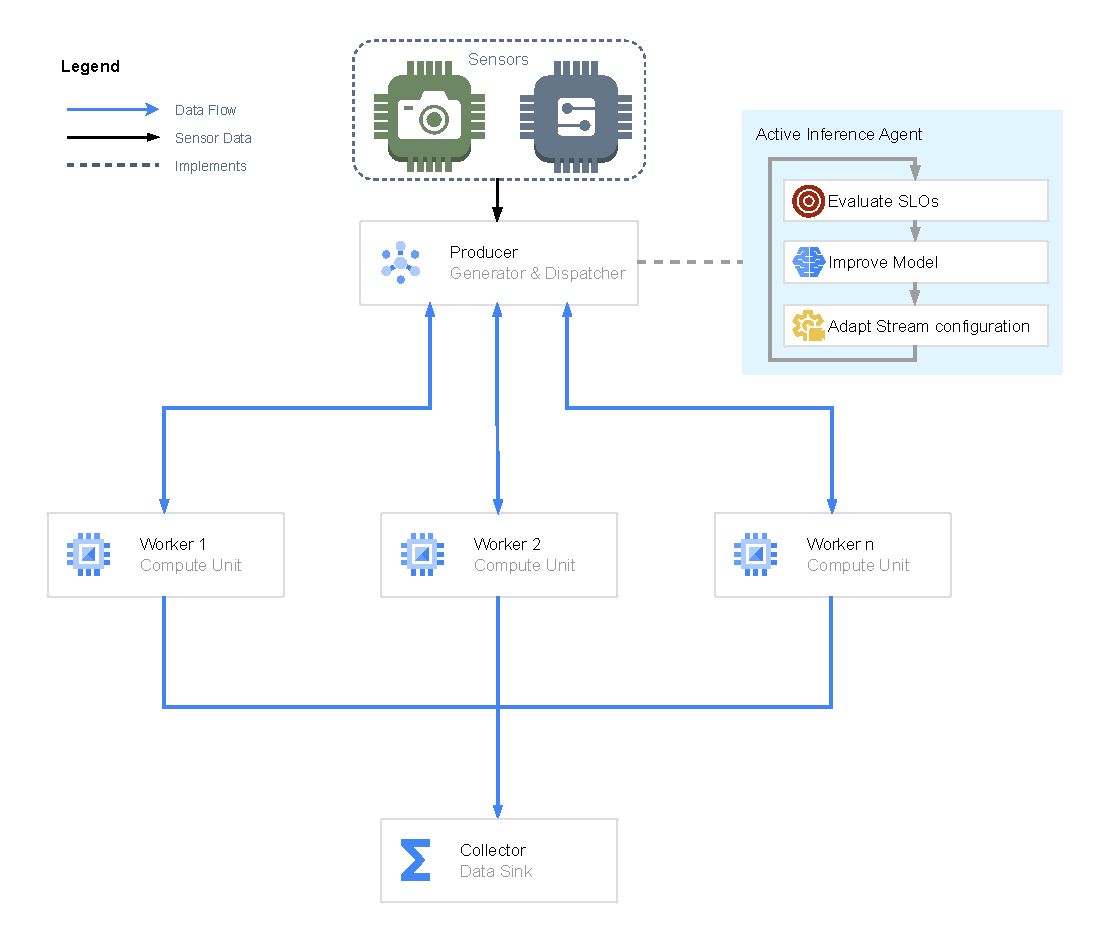
\includegraphics[width=\textwidth]{img/methodology_parallel_pipeline_overview.drawio.pdf}
    \caption{Overview of system architecture}
    \label{fig:parallel-distributed-pipeline}
\end{figure}


\subsection{Task Distribution and Load Balancing}
Tasks are distributed in a decentralized fashion: each worker node actively requests tasks when ready to compute, forming a pull-based load balancing model. This mechanism enables the system to scale to a large number of workers without requiring global synchronization. This load-balancing pattern emerges naturally as faster or less burdened nodes consume more tasks \cite{estrada_comparing_2015}.

While such an architecture increases communication overhead, as the worker node has to go out of its way to request data, it also enables efficient utilization of heterogeneous compute resources by aligning task assignment with runtime capacity.

\subsection{Asynchronous Communication Model}
All communication between components is asynchronous. Producers dispatch tasks without blocking \cite{lauener_how_2018}; workers process and return results independently; and collectors operate on incoming data streams without waiting on global completion barriers.

This asynchronous design supports robustness under dynamic conditions, such as fluctuating task loads or varying network bandwidth \cite{nguyen_octopinf_2025}. This non-blocking operation is critical for real-time scenarios in which latency constraints must be maintained regardless of individual node performance fluctuations.

\section{Service Level Objectives for Resource Management}
Each SLO defines a desired operational range for a specific performance metric. They are represented as bounded variables whose values must remain within a target range to ensure system stability.

For instance, an SLO limiting memory usage might be formulated as:
\[
\text{Memory} < \theta
\]

Where \(\theta\) denotes the predefined threshold for acceptable memory capacity, e.g., \(\theta = 512\text{MB}\). Violating this constraint signals that the system is exceeding its limitations and requires an elastic adjustment.

In this thesis, SLOs are implemented through a normalized ratio between the current observation $x$ and the associated threshold $\theta$. This ratio, hereafter referred to as the \textit{SLO value}, is computed as

\[
\text{SLO value} = \frac{x}{\theta}
\]

An SLO value less than 1 indicates that the constraint is fulfilled. Conversely, values exceeding 1 
(\(\geq1\)) signal an SLO violation, necessitating corrective action.

For illustration, consider again the memory usage constraint with \(\theta = 512\text{MB}\). A current observation of \(x = 256\text{MB}\) yields an SLO value of \(0.5\), thus satisfying the objective. In contrast, a usage of \(x = 523\text{MB}\) results in

\[
\text{SLO value} = \frac{523}{512} \approx 1.02
\]
indicating a minor SLO violation.

This formulation enables a uniform treatment of heterogeneous resource constraints, allowing the system to monitor, compare, and respond to SLO fulfillment in a principled and quantitative manner.

\subsection{Multi-Dimensional Elasticity}
Due to the resource-constrained nature of edge computing environments, vertical or horizontal scaling techniques cannot be used to uphold SLOs. To fulfill SLOs, the system must dynamically adapt the computational demand to fit the system's resource budget, meaning specific parameters need to be modifiable during runtime.

This requires that each stream processing task supports multiple execution configurations, each with associated performance characteristics and requirements. A configuration defines a set of \textit{stream quality parameters}, such as inference quality, task frequency and task size. All of these parameters directly impact QoE and computational demands. The system supports multi-dimensional elasticity, meaning that these parameters can be individually tuned during runtime.

The Producer operates as the central controller of stream parameterization. The changing of stream parameter can be separated into two types:

\begin{itemize}
    \item \textbf{Task generation:} Stream parameters that directly affect the generation of tasks are changed directly at the producer level. The configuration then affects all newly generated tasks.
    \item \textbf{Task processing:} Stream parameters that affect large changes on the worker, such as switching inference quality, require coordination between producer and worker. When the producer dictates a change, it enqueues a control task, detailing the nature of the change, in the \textit{backlog}\label{def:backlog} of each worker. The next time a worker requests a task from the producer, it receives the control tasks and makes the described changes, before continuing with normal stream processing. This ensures synchronized configuration among workers.
\end{itemize}

\section{Active Inference-Based Elasticity Control}
The system exposes control of the \textit{stream quality parameters} to the AIF agent.
\subsection{Generative Model Construction}
Central to a capable AIF agent is the construction of the \textit{generative model}. It represents the causal relationships between system configuration parameters and observable SLO metrics. It captures both direct (i.e., quality parameters) and indirect dependencies (i.e., SLO) affecting agent behavior. This model includes:
\begin{itemize}
  \item \textbf{Observation model \(P(o \mid s)\):} Obeservations of Stream Paramters and SLO values.
  \item \textbf{Transition model \(P(s_{t+1} \mid s_t,a_t)\):} Actions taken by Agent to change stream quality paramters.
  \item \textbf{Prior preferences over observations \(P(o)\):} Agent prefers high stream quality paramters, while strongly averting unfilled SLOs.
  \item \textbf{Prior beliefs about hidden states \(P(s_0)\):} The initial state of SLOs and stream quality parameters, before any data has been processed.
  \item \textbf{Prior beliefs about policies: \(P(\pi)\):} 
\end{itemize}

\subsubsection{Prioritization Strategy}
Crucially, the SLOs and \textit{stream quality parameters} are encoded as prior preferences with different absolute values. The preference to fulfill an SLO must be stronger than the preference to increase the quality of the stream (i.e., increase computational demand). This results in a lexicographic prioritization, where the primary objective is to maintain SLOs and the secondary objective of maximizing \textit{stream quality parameters}. This prioritization reflects the insight that QoE directly correlates with increased computational cost. Therefore, aggressive maximization of \textit{stream quality parameters} without constraint awareness would lead to SLO violations and system degradation.

The relationship between configuration and SLO fulfillment is non-linear. Therefore, the system must learn which configurations fulfill SLOs under which conditions, and which trade-offs are most efficient \cite{sedlak_towards_2025}.

\subsection{Continous Observation and Configuration Adjustment}
The AIF loop~\ref{sec:active-inference-loop} is executed periodically during the producer's runtime to evaluate and adapt the system's configuration. Finding an appropriate interval between evaluations is critical, as it determines how frequently the agent can revise and apply its control policy. Short intervals (e.g., 50\,ms) allow rapid responsiveness but risk instability. Actions may be issued faster than their causal effects can propagate through the system, leading to overcompensation or oscillatory behavior. This is especially problematic in stream processing pipelines where SLO-relevant variables such as memory usage evolve with delay. Conversely, overly long intervals (e.g., 5\,s) hinder the system’s ability to respond to rapid environmental changes, potentially causing SLO violations due to latency in corrective actions. The implementation in chapter~\ref{chap:implementation} executes an action-perception cycle every 500\,ms.

\subsubsection{Active Inference Loop}
Each iteration of the loop involves a three-step procedure: observation, state and policy inference, and action sampling.

This sub-section describes the cycle based on the \texttt{pymdp} \cite{heins_pymdp_2022}, a python library implementing AIF for Markov Decision Processes. It serves as a great abstraction for this explanation and is later utilized in the implementation~\ref{sec:evaluation-implementation-active-infernce-agemt}. This choice does not constrain the generality of the proposed methodology. The loop structure, model components, and control logic are independent of any specific framework and can be implemented using alternative tools or custom inference routines. However, \texttt{pymdp} offers a modular and transparent interface for constructing Active Inference agents in discrete state spaces, well-suited to the modeling assumptions underlying this work. Its use in this thesis serves both as a practical vehicle for experimentation and as a clear reference implementation of the conceptual model described. 

\begin{enumerate}
    \item \textbf{Observation Sampling (Peception):} The agent receives updated observations from the environment via the Producer. These include current values for the stream quality parameters and the normalized SLO values. The observations are then encoded in \(o_t\).

    \item \textbf{Belief Updating over States and Policies:} The agent updates its beliefs about hidden states $s_t$ using the latest observation \(o_t\), applying variational Bayesian inference to approximate the posterior \(Q(s_t)\). This is handled via:
    \begin{quote}
        \texttt{agent.infer\_states(\(o_t\))}
    \end{quote}
    Subsequently, the agent infers a posterior distribution over policies $\pi$, each representing a sequence of actions (e.g., changing inference quality) over a receding horizon. Policies are evaluated by their expected free energy $\mathbb{G}(\pi)$, which integrates both \emph{epistemic value} (information gain) and \emph{instrumental value} (goal fulfillment). Policies minimizing expected free energy are preferred. This step is implemented via:
    \begin{quote}
        \texttt{agent.infer\_policies()}
    \end{quote}
     Policies that minimize anticipated SLO violations while improving QoE are preferred.

     In addition, the agent updates its generative model by refining its beliefs about the observation and transition probabilities through
    \begin{quote}
        \texttt{agent.update\_A(\(o_t\))} \\
        \texttt{agent.update\_B(\(Q(s_t)\))}
    \end{quote}
    
    \item \textbf{Action Selection:} The agent samples the most promising action from the posterior over policies and executes the first action in the sequence. This corresponds to reconfiguring the stream pipeline by adjusting stream parameters. Execution is performed via:
    \begin{quote}
        \texttt{action = agent.sample\_action()}
    \end{quote}
    The action is then translated into a concrete command that is either applied to the task generation template or inserted as a control task into the worker backlog (see Section~\ref{def:backlog}).
\end{enumerate}

\subsubsection{Homeostasis}
The agent's long-term objective is the persistent minimization of \textit{surprise} \cite{sedlak_adaptive_2024}, achieving homeostasis. This is done by finding a configuration that maximizes QoE, while upholding all SLOs.